\section{Implementation}
\label{sec:implementation}

\begin{figure}[t]
\begin{centering}
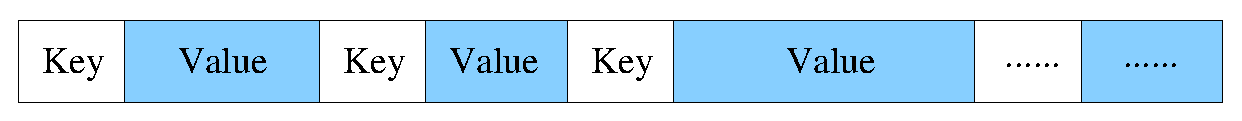
\epsfig{file=figures/sstable.eps,width=1.00\linewidth}
\caption{SSTable}
\label{fig:sstable}
\end{centering}
\end{figure}

\begin{figure}[t]
\begin{centering}
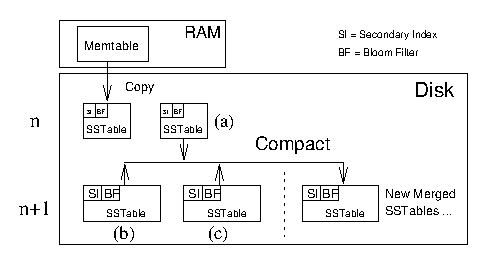
\epsfig{file=figures/leveldb-compact.eps,width=1.00\linewidth}
\caption{LevelDB Compaction}
\label{fig:compact}
\end{centering}
\end{figure}

We implemented MRIS using LevelDB~\cite{leveldb-web}, an open source
key/value database engine developed by Google. LevelDB is
log-structured and organizes data into Sorted String Table (SSTable).
SSTable, introduced in Bigtable~\cite{chang06osdi}, is an immutable
data structure containing a sequence of key/value pairs sorted by the
key as shown in Figure~\ref{fig:sstable}. Besides key and value, there
might be optional fields such as CRC, compression type etc. SSTable
are mostly saved as files and each of them can contains data
structures, such as bloomfilter, to facilitate key lookup. SSTable
have counterpart in the memory called Memtable. The key/value pairs in
Memtable are often kept in data structures easy for insert and lookup
such as red/black tree and skiplist.

LevelDB, as well as most other key/value engines, use Log-Structured
Merge Trees (LSM)~\cite{lsm} for internal storage. When key/value
pairs are first added, they are inserted into Memtable.  Once the size
of the Memtable growes beyond a certain threshold, the whole Memtable
is flushed out into a SSTable, and a new Memtable is created for
insertion. When key/value pairs get changed, the new pairs are
inserted without modifying the old pairs. When a key/value pair is
deleted, a marker of the deletion is inserted by setting a flag inside
the key called \texttt{KeyType}. This way key/value can provide large
insertion throughput because data is written out using sequential
I/Os, which have good performance on Hard Disk Drives (HDD). 

To serve a key lookup, Memtable is queried firstly. If not found in
Memtable, the SSTables are queried in reverse chronological order. A
naive implementation of such a lookup can be very slow because the
whole database need be read and checked in the worst case. To make
lookup fast, SSTable are organized into several layers with the size
of each table increasing from the top layer to the bottom. Background
jobs are launched periodically to sort and merge small SSTables into
larger ones in the next layer. This is called compaction. Deleted
pairs are also removed during compaction. Then a lookup iterates the
SSTables layer by layer and returns once the key is found.  Because
SSTables are sorted by key, it enables fast lookup algorithm like
binary search. There is also index for SSTables tells the key range
covered by a particular SSTable so that it suffice just checking the
SSTables whose key ranges cover the interested key. Inside each
SSTable, we can have a bloomfilter to filter negative key lookup and a
secondary index for faster search.

In LevelDB, there are two Memtables, once one is filled, the other one
is used for further insertion. The filled one is flushed into a
Memtable in background. Its compaction procedure is illustrated in
Figure~\ref{fig:compact}. One SSTable (a) at layer $n$ is merged with
the SSTables at layer $n+1$ that have overlapping keys with (a) into
new SSTables at layer $n+1$.

A drawback of compaction is that pairs are read and written multiple
times when they are gradually merged from the top layer to the bottom.
Although compaction is scheduled in background, it still influences
the overall system performance when the I/O traffic is heavy. Reads
and writes of large pairs make compaction long and in turn introduce
more negative effect on performance. Therefore, it is desirable to
reduce the copying of large pairs. Because the log-structured nature
of key/value store, once written, the pairs will never be updated. So
it is reasonable to keep large values unmoved especially when the
reduce of data copying can offset the cost of an extra disk seek.

As cloud computing is spreading widely, high throughput storage system
is required because, in consolidated cloud environment, data are
generated fast in great volume. It demands not only high storage
throughput but also large capacity. It is a natural choice to
compromise between cost and performance and save different data on
different media. Some companies achieved this using big memory for hot
data and storing not-so-hot data into second-level
storage~\cite{level_lifetime}.  However, memory is expensive and
volatile. New NVRAM storage media such as Flash SSD provides an
alternative solution, which can be cheaper and safer.

\begin{figure}[t]
\begin{centering}
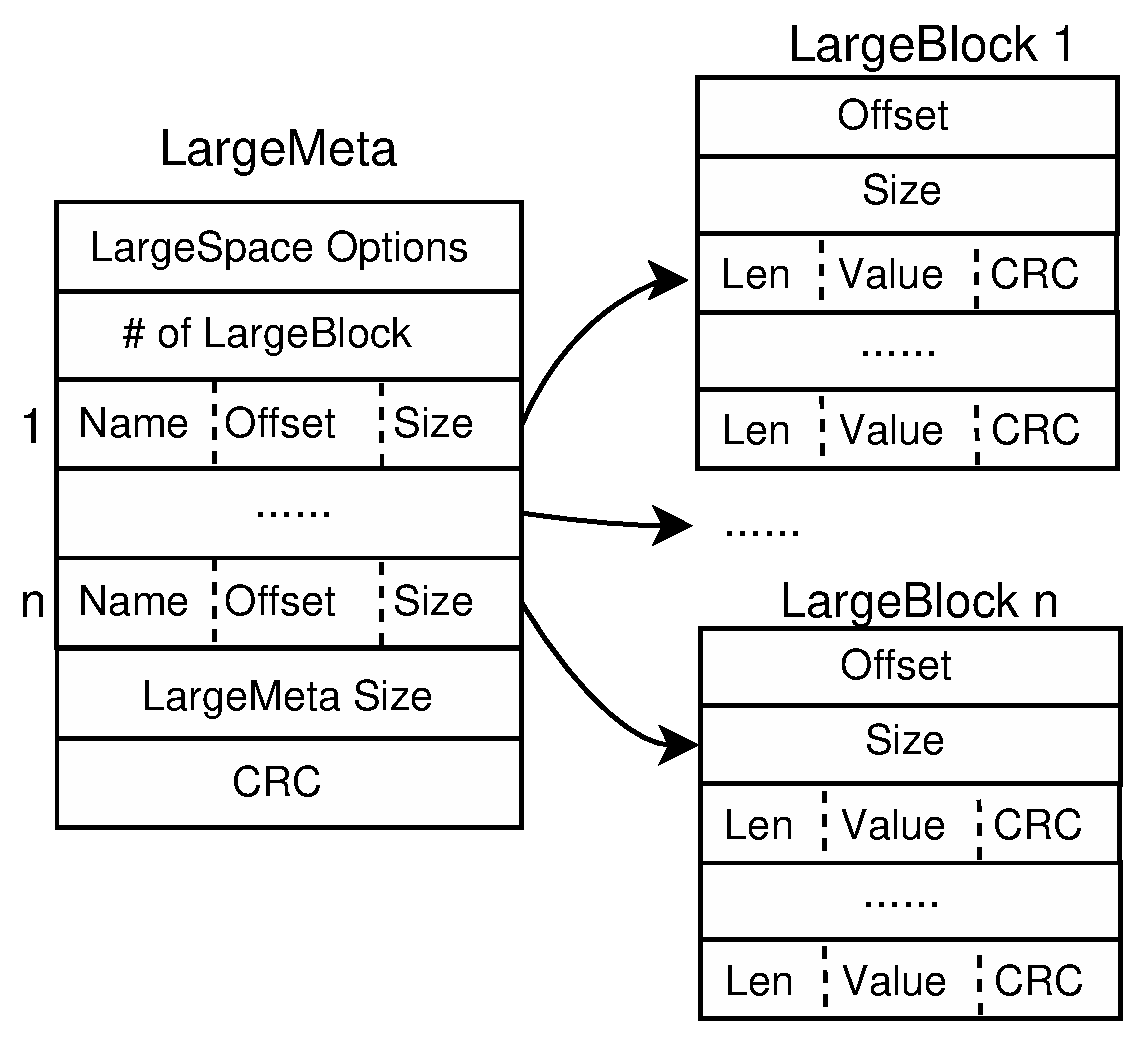
\epsfig{file=figures/large-space.eps,width=1.00\linewidth}
\caption{Large Space}
\label{fig:space}
\end{centering}
\end{figure}

Based on the idea of saving different data on different media, we
modify LevelDB to save large values separately into a space called
LargeSpace. LargeSpace is essentially a log and can be saved in media
different from the SSTables. Upon a request of insertion, the value is
appended into LargeSpace and an address is returned. The address is
used for later retrieve of the value. To ease management, LargeSpace
is splited into files called LargeBlocks. The threshold of split,
called SplitThreshold, is a configurable parameter with a default
value of 64MB. Although LargeSpace is splited, we enforce that no
value will be splited among LargeBlocks. Therefore, it is possible
that a LargeBlock is larger than the split threshold if there is a
huge value in that LargeBlock.  LargeBlocks are recorded in a metadata
file called LargeMeta. The formats of LargeMeta and LargeBlock and
their relationship is illustruated in Figure~\ref{fig:space}.

It is worth notice that LargeMeta is an immutable file. A new one is
created every time it is updated. LargeMeta can be readily rebuilt
using information from LargeBlocks. Many versions of LargeMeta are
kept which provides a natural support for versioning. This makes the
metadata resistent to harzardous situations such as system crash and
file corruption.

\begin{figure}[t]
\begin{centering}
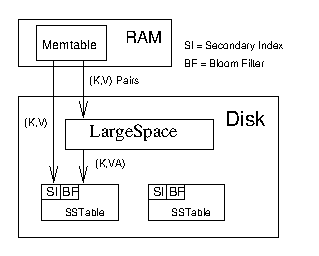
\epsfig{file=figures/mris-store.eps,width=1.00\linewidth}
\caption{MRIS Insertion.}
\label{fig:mrisinsert}
\end{centering}
\end{figure}

A key/value is considered to be large and will be saved in LargeSpace
when its value size is larger than a configurable threshold, named
SizeThreshold. SizeThreshold provides a simple but effective knob to
tradeoff between cost and performance when LargeSpace and SSTable are
stored in different places. We plan to use more sophisticated
algorithm to determine where to place a certain pair considering not
only size but also hotness and access pattern.

Insertion of MRIS is illustruated in Figure~\ref{fig:mrisinsert}.
When key/value pairs are firstly inserted into Memtable, they are
treated equally. Large pairs in a Memtable are checked when the
Memtable becomes full and is dumped into SSTable. Whereas small pairs
go to SSTable without touch, the value of large pairs are firstly
inserted into LargeSpace. For each large pair, a new pair is formed
and inserted into SSTable. The key of the new pair is the same as the
old key except its \texttt{KeyType} is changed to indicate that it
represents a large pair.  The value of the new pair contains the size
of the original value, and its addresses in LargeSpace.

%%%%%%%%%%%%%%%%%%%%%%%%%%%%%%%%%%%%%%%%%%%%%%%%%%%%%%%%%%%%%%%%%%%%%%%%%%%%%%
%% For Emacs:
% Local variables:
% fill-column: 70
% End:
%%%%%%%%%%%%%%%%%%%%%%%%%%%%%%%%%%%%%%%%%%%%%%%%%%%%%%%%%%%%%%%%%%%%%%%%%%%%%%
%% For Vim:
% vim:textwidth=70 noai nocin nosi
%%%%%%%%%%%%%%%%%%%%%%%%%%%%%%%%%%%%%%%%%%%%%%%%%%%%%%%%%%%%%%%%%%%%%%%%%%%%%%
% LocalWords:  SSTable LevelDB Memtables
